\chapter{Description générale}

\section{Environnement du projet}
Pour ce projet, je me base sur le code de mon encadrant, qui résout le sous-problème où l'ordre de réalisation des jobs et la constitution des lots sont fixés.
Le code est écrit en C++ avec Visual studio 2017 et utilise la bibliothèque Cplex.

Le projet existant utilise des fonctionnalités de Visual c++ et n'est pas compatible avec le C++ standard,
 une partie de mon travail consiste à l'adapter.
\section{Caractéristiques des utilisateurs}
Il s'agit d'un projet de recherche, les utilisateurs seront des chercheurs souhaitant tester les algorithmes développés dans ce projet.
 
\section{Fonctionnalités du système}
Les applications développées dans ce projet ont pour objectif de comparer plusieurs méthodes de résolution du problème défini précédemment.
Pour cela, deux méthodes de résolutions sont testé,  une méthode exacte utilisant un solveur et une recherche locale.
Pour permettre de comparer les méthodes, elles utilises la même structure de données pour les instances et les solution.


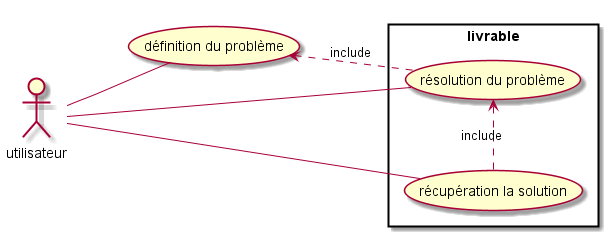
\includegraphics[width=\textwidth]{parts/description_generale/use_cases}

Les implémentations des méthodes donnent deux applications distinctes, utilisant une même bibliothèque qui définit les structures de données du problème.
Les exécutables s'exécutes en console et prennent en paramètre le chemin vers le fichier d'instance et
le chemin vers le fichier où écrire les résultats.
Les résultats sont écrit en JSON et inclue des données tel que la durée de la résolution.
L'utilisation du format JSON permet d'exploiter facilement les résultats avec de nombreux outils.


\section{Structure générale du système}

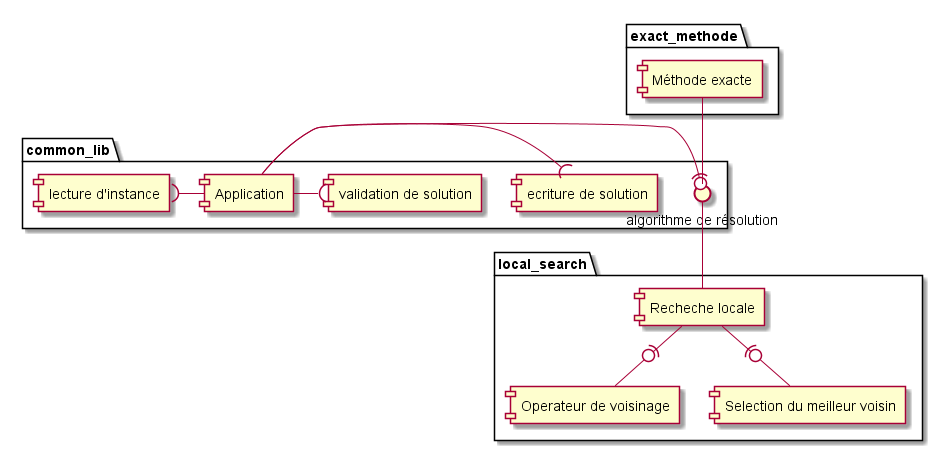
\includegraphics[width=\textwidth]{parts/description_generale/composants}